\section{Results – Strategy S3: Multi-LLM Consensus (Full)}
\label{sec:eval-s3}

The \textbf{S3: Multi-LLM Consensus (Full)} strategy runs multiple LLMs on the full document and aggregates with a verification/consensus step.
We evaluate three variants:
\textbf{S3.0} = no few-shot examples on the original MUC-4 dataset;
\textbf{S3.1} = with few-shot examples on the original dataset;
\textbf{S3.2} = with few-shot examples on a speech-style variant.

\subsection*{Headline Results}

% Add to your preamble:
% \usepackage{pgfplots}
% \pgfplotsset{compat=1.18}

\begin{figure}[H]
\centering
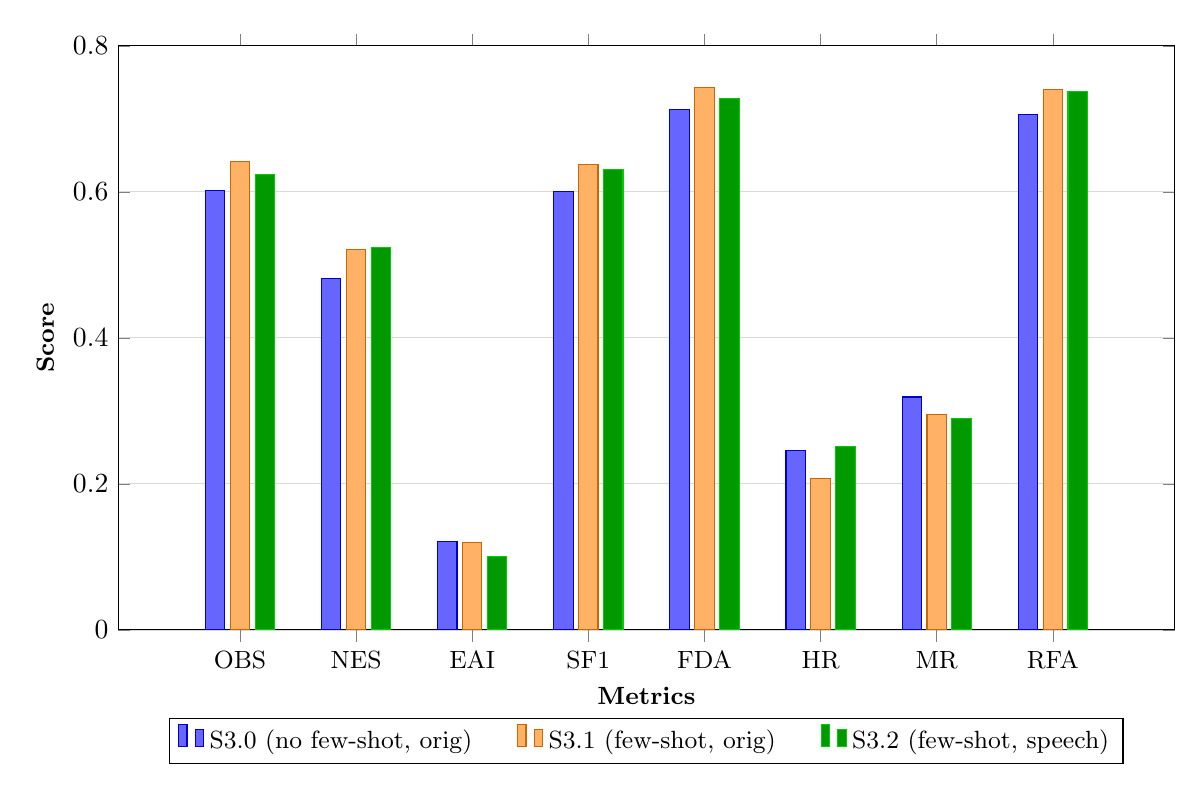
\begin{tikzpicture}
  \begin{axis}[
    width=15cm,
    height=9cm,
    ybar,
    bar width=7pt,
    ylabel={Score},
    ylabel style={font=\small\bfseries},
    xlabel={Metrics},
    xlabel style={font=\small\bfseries},
    symbolic x coords={OBS, NES, EAI, SF1, FDA, HR, MR, RFA},
    xtick=data,
    xticklabel style={font=\small},
    ymin=0,
    ymax=0.8,
    ytick={0, 0.2, 0.4, 0.6, 0.8},
    ymajorgrids=true,
    grid style={line width=0.3pt, draw=gray!30},
    legend style={
      at={(0.5,-0.15)},
      anchor=north,
      legend columns=3,
      font=\small,
      /tikz/every even column/.append style={column sep=0.5cm}
    },
    enlarge x limits=0.15,
  ]
  
  % S3.0 (no few-shot, orig) - Blue
  \addplot[fill=blue!60, draw=blue!80!black] coordinates {
    (OBS, 0.602)
    (NES, 0.481)
    (EAI, 0.121)
    (SF1, 0.601)
    (FDA, 0.713)
    (HR, 0.246)
    (MR, 0.319)
    (RFA, 0.706)
  };
  \addlegendentry{S3.0 (no few-shot, orig)}
  
  % S3.1 (few-shot, orig) - Orange
  \addplot[fill=orange!60, draw=orange!80!black] coordinates {
    (OBS, 0.641)
    (NES, 0.521)
    (EAI, 0.120)
    (SF1, 0.638)
    (FDA, 0.743)
    (HR, 0.208)
    (MR, 0.295)
    (RFA, 0.740)
  };
  \addlegendentry{S3.1 (few-shot, orig)}
  
  % S3.2 (few-shot, speech) - Green
  \addplot[fill=green!60!black, draw=green!80!black] coordinates {
    (OBS, 0.624)
    (NES, 0.524)
    (EAI, 0.100)
    (SF1, 0.630)
    (FDA, 0.728)
    (HR, 0.251)
    (MR, 0.289)
    (RFA, 0.738)
  };
  \addlegendentry{S3.2 (few-shot, speech)}
  
  \end{axis}
\end{tikzpicture}
\caption{Headline metrics for S3 variants on MUC-4 ($N{=}100$).}
\label{fig:s3-variants-bar}
\end{figure}


\paragraph{Per-field (reference for S3.1).}
Consensus is strong for \texttt{perpetratorOrganization} and \texttt{weapon}; \texttt{perpetratorIndividual} remains hardest; \texttt{incidentLocation} improves vs.\ single-pass.

\begin{table}[H]
    \centering
    \caption{Per-field average scores for S3.1 ($N{=}100$).}
    \label{tab:s3-perfield}
    \begin{tabular}{lcc}
        \toprule
        Field & Avg.\ Score & \#Docs \\
        \midrule
        incidentType & 0.510 & 100 \\
        incidentDate & 0.730 & 100 \\
        incidentLocation & 0.554 & 100 \\
        incidentStage & 0.730 & 100 \\
        perpetratorIndividual & 0.561 & 100 \\
        perpetratorOrganization & 0.756 & 100 \\
        target & 0.570 & 100 \\
        victim & 0.567 & 100 \\
        weapon & 0.793 & 100 \\
        \midrule
        \textbf{Overall (OBS)} & \textbf{0.641} & \textbf{900 comps} \\
        \bottomrule
    \end{tabular}
\end{table}

\subsection*{Latency}

\begin{figure}[H]
\centering
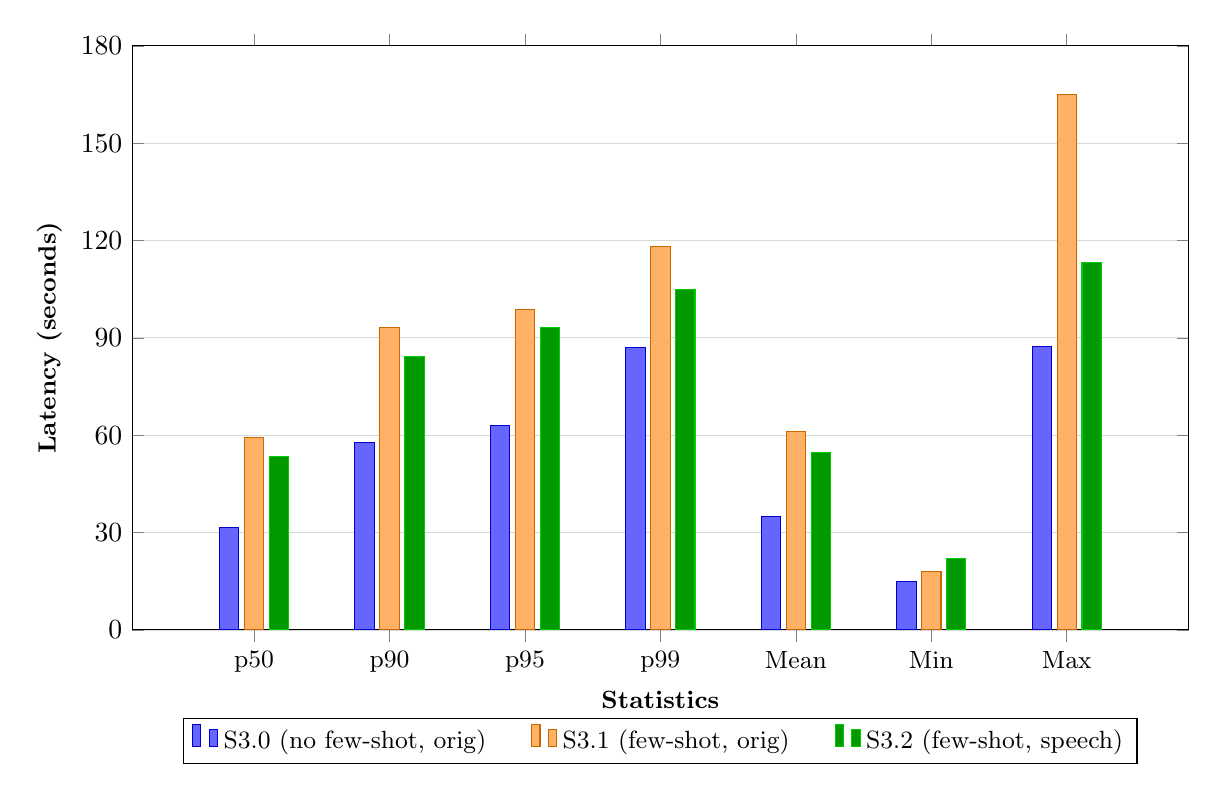
\begin{tikzpicture}
  \begin{axis}[
    width=15cm,
    height=9cm,
    ybar,
    bar width=7pt,
    ylabel={Latency (seconds)},
    ylabel style={font=\small\bfseries},
    xlabel={Statistics},
    xlabel style={font=\small\bfseries},
    symbolic x coords={p50, p90, p95, p99, Mean, Min, Max},
    xtick=data,
    xticklabel style={font=\small},
    ymin=0,
    ymax=180,
    ytick={0, 30, 60, 90, 120, 150, 180},
    ymajorgrids=true,
    grid style={line width=0.3pt, draw=gray!30},
    legend style={
      at={(0.5,-0.15)},
      anchor=north,
      legend columns=3,
      font=\small,
      /tikz/every even column/.append style={column sep=0.5cm}
    },
    enlarge x limits=0.15,
  ]
  
  % S3.0 (no few-shot, orig) - Blue
  \addplot[fill=blue!60, draw=blue!80!black] coordinates {
    (p50, 31.47)
    (p90, 57.79)
    (p95, 63.02)
    (p99, 87.16)
    (Mean, 34.83)
    (Min, 14.85)
    (Max, 87.24)
  };
  \addlegendentry{S3.0 (no few-shot, orig)}
  
  % S3.1 (few-shot, orig) - Orange
  \addplot[fill=orange!60, draw=orange!80!black] coordinates {
    (p50, 59.39)
    (p90, 93.15)
    (p95, 98.77)
    (p99, 118.28)
    (Mean, 61.09)
    (Min, 18.13)
    (Max, 164.96)
  };
  \addlegendentry{S3.1 (few-shot, orig)}
  
  % S3.2 (few-shot, speech) - Green
  \addplot[fill=green!60!black, draw=green!80!black] coordinates {
    (p50, 53.45)
    (p90, 84.15)
    (p95, 93.31)
    (p99, 104.99)
    (Mean, 54.55)
    (Min, 22.01)
    (Max, 113.26)
  };
  \addlegendentry{S3.2 (few-shot, speech)}
  
  \end{axis}
\end{tikzpicture}
\caption{Latency statistics for S3 variants (seconds).}
\label{fig:s3-latency-bar}
\end{figure}

\subsection*{Insights}

\begin{itemize}
    \item \textbf{Consensus cuts hallucinations and improves calibration.} Relative to iterative S2.1, S3.1 lowers HR (0.301$\rightarrow$0.208) and raises FDA (0.718$\rightarrow$0.743), with higher OBS (+0.022) at a modest MR increase (0.267$\rightarrow$0.295). This reflects better confidence alignment from cross-model agreement.
    \item \textbf{Competitive with the best single-pass accuracy.} Against S1.1, S3.1 is close on OBS (0.641 vs.\ 0.644) but improves NES (0.521 vs.\ 0.504), suggesting stronger content quality on gold-nonempty fields; MR also improves (0.295 vs.\ 0.313), while HR is slightly higher than S1.1’s very conservative rate (0.208 vs.\ 0.180).
    \item \textbf{Speech-style robustness holds.} S3.2 maintains NES leadership among S3 variants (0.524) and strong RFA (0.738), with MR the lowest (0.289). Compared to S1.2, S3.2 trades a small OBS deficit (0.624 vs.\ 0.626) for better NES (+0.016) and similar FDA (0.728 vs.\ 0.727).
    \item \textbf{Field patterns persist.} \texttt{perpetratorOrganization}/\texttt{weapon} remain easiest; \texttt{perpetratorIndividual} continues to lag due to sparse, ambiguous references; \texttt{incidentLocation} benefits from full-context cross-checking (S3.1: 0.554 baseline) vs.\ S1’s single pass.
    \item \textbf{Latency cost is real but tails are reasonable.} S3.1 has higher median and mean than S1.1, yet a shorter extreme tail than S1.1 (p99 118.3\,s vs.\ 134.9\,s). S3.0 offers a faster consensus baseline when few-shot is unavailable.
\end{itemize}
